\documentclass[a4paper]{article}

\usepackage[english]{babel}
\usepackage{amsmath}
\usepackage{graphicx}
%\usepackage{algorithm}
%\usepackage{algorithmic}
%\usepackage{algpseudocode}
\usepackage{url}


\title{Omega3P+PUMI Progress Report}

\author{Cameron W. Smith, Gerrett Diamond}

\date{\today}

\begin{document}
\maketitle

\section{In-memory Integration}

Parallel simulations on massively parallel systems are most effective when data
movement is minimized.
Data movement costs increase with the depth of the memory hierarchy; a design
trade-off for increased capacity.
For example, the highest level on-node storage in the IBM BlueGene/Q A2
processor~\cite{haring2012ibm} is the per-core 16KiB L1 cache (excluding
registers) and has a peak bandwidth of 819 GiB/s.
The lowest level on-node storage, 16GiB of DDR3 main memory, provides a million
times more capacity at the cost of 19 times less bandwidth,
43GiB/s~\cite{lo2014roofline}.
One level further down the hierarchy is the parallel filesystem
~\footnote{We assume, for the sake of simplicity, that the main memory of other nodes is not
available.
In practice, most applications do not not use all the on-node memory and some
checkpoint-restart methods take advantage of this for increased performance
~\cite{rma-fault-tolerance-2014,isaila2014making,compression-cr-2012}.
}.
At this level the bandwidth and capacity relationship is less clear as the
filesystem is a shared resource.
Table~\ref{tbl:systems} lists the per-node peak main memory and filesystem
bandwidth across four generations of Argonne National Laboratory leadership
class systems: BlueGene/L~\cite{yu2006high,adiga2002overview}, Intrepid
BlueGene/P~\cite{lang2009performance,alam2008early}, Mira
BlueGene/Q~\cite{haring2012ibm,bui2014scalable}, and 2018's
Aurora~\cite{aurorafacts}.
Based on these peak values the bandwidth gap between main memory and the
filesystem is at least three orders of magnitude.
Software must leverage the cache and main memory bandwidth performance advantage
during as many operations as possible to maximize performance.

\begin{table}[h]
\centering
\caption{Per-node main memory and filesystem peak bandwidth over four
  generations of Argonne National Laboratory systems.
  The values in parentheses indicate the increase relative to
  the previous generation system.}
\label{tbl:systems}
\begin{tabular}{l|cc}
        & Memory BW & Filesystem BW \\
        & (GiB/s)    & (GiB/s)    \\
 \hline
 BG/L   & 5.6       & 0.0039         \\
 BG/P   & 14 (2.4x) & 0.0014 (0.36x)   \\
 BG/Q   & 43 (3.1x) & 0.0049 (3.5x) \\
 Aurora & 600 (14x) & 0.020 (4.1x)
\end{tabular}
\end{table}

Approaches for high performing and scalable component interactions avoid
file-based I/O through in-memory data streams and component functional
interfaces.
The ADIOS tools provide an alternative mechanism for the in-memory coupling of
executables~\cite{bennett2012combining,zhang2012enabling}; our work here focuses
on the interaction of libraries operating within the same process.
Components that support a common file format can use our data stream approach
with minimal software changes to exchange data via memory buffers instead of files.
This approach is also a logical choice for legacy analysis codes that do not
provide functional interfaces to access or create their input and output data
structures.

Components with functional interfaces that encapsulate creation, deletion, and
access to underlying data structures support in-memory interactions.
The level of interface granularity selected for defining interactions has a
proportional impact on flexibility and development costs.
At a very fine level a developer may implement all mesh entity query functions such
that components can share the same mesh structure; trading increased development
costs for lower runtime memory usage.
An excellent example of this is the use of octree structures in the
development of parallel adaptive analyses~\cite{BursteddeWilcoxGhattas11}.
At a coarser level a developer may simply create another mesh
representation through use of interfaces encapsulating mesh construction;
trading higher runtime memory usage for lower development costs.
For example, an existing solver component can embed low level
calls to mesh-entity iterators~\cite{Ollivier10}.
Although this method will allow for in-memory integration, it suffers from the
same disadvantages as a tightly coupled approach in that a significant amount of
time and effort will be required for code modification and verification.
A generalization of this coarser level approach defines common sets of
interfaces through which all components interact.
For example, in the rotorcraft aerodynamics community the HELIOS platform
provides a set of analysis, meshing, adaptation, and load balancing components
via the Python-based Software Integration Framework~\cite{sankaran2010application}.

Our implementation of in-memory integration for PUMI and Omega3p uses
mesh query and construction APIs for mesh and field conversion combined with
fine-level APIs for querying higher-order geometric data for element
integrals.
The mesh conversion approach trades code simplicity for increased peak memory usage.
During PUMI adaptation and load balancing only the PUMI mesh is stored.
After conversion though, we store both the PUMI mesh and the Omega3P
DistMesh.
Mesh conversion alone is not sufficient to integrate over elements near the
geometric boundary.
We support these integrals by implementing Omega3P geometric queries with PUMI
APIs that can interrogate parametric model information provided by CAD
kernels.

\section{Load Balancing}\label{sec:lb}

The Omega3P solving step relies on both on part mesh entities as well as a layer of 
ghosted elements along each part boundary. Figure \ref{fig:ghost3} shows an 
example of a mesh with three layers of ghosting. In order to reach maximum efficiency
for ghost-based codes partitioning must target minimizing the sum of the 
weights of ghosted and non-ghosted elements as well as the mesh entities holding
degrees-of-freedom.

\begin{figure}[ht]
\centering
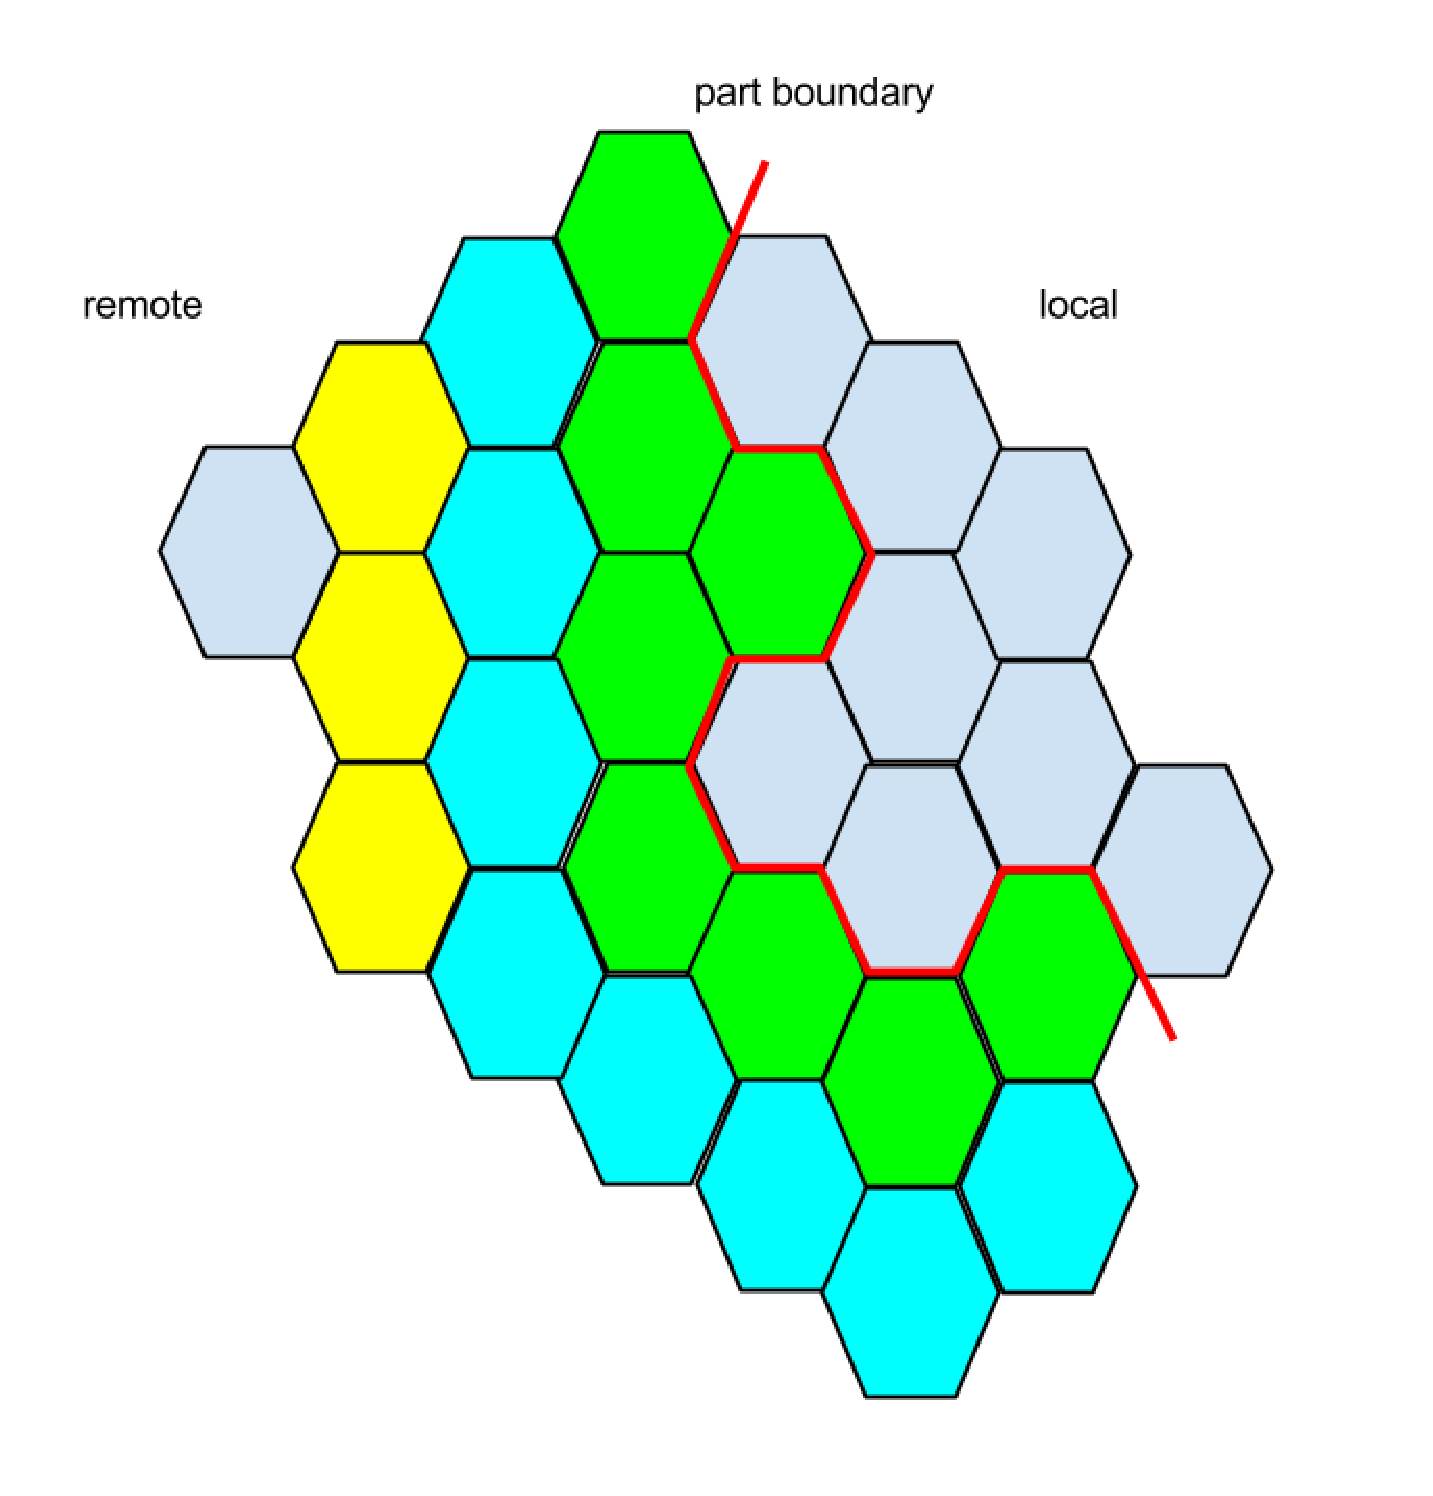
\includegraphics[width=0.4\textwidth]{ghostingExample.eps} 
\caption{\label{fig:ghost3} Three layers of elements ghosted from the remote part to the local part.  The first layer is colored green, the second blue, and the third yellow.}
\end{figure}

Given a
uniformly-weighted mesh we first partition it one part to $N$ parts using
Zoltan's interface to ParMETIS's multi-level graph-based method.
Once distributed we then run ghost-aware diffusive load balancing using
ParMA~\cite{SmithParma2015} to get a final mesh that is well balanced for
analysis procedures.
ParMA's partition improvement procedures account for
the ghosted layers using a combination of existing element selection criteria
and an extended `weight' tracking mechanism.
The weight tracking extension relies on the exact knowledge of the change to the
ghosted elements as elements on a heavy part are selected for migration to a
light part.
To accurately accommodate for Omega3P's ghosting we will be extending ParMA's
ghosting to be able to balance element-based ghosts; our current
workflow reuses an existing ParMA vertex-based ghost balancer.
In addition to balancing ghosts, ParMA also needs to account for the
degree-of-freedom holders defined by the use of hierarchical Nedelec basis
functions~\cite{ingelstrom2006new}.
For first order elements this requires balancing edges.
Second order elements requires edges and faces, and above that edges, faces, and
regions need to be balanced.

\section{Status}
Omega3P now supports reading a curved mesh from a NetCDF formatted file into a
DistMesh, or reading a PUMI mesh directly.
If a serial DistMesh was read it is converted to a PUMI-APF mesh and then 
partitioned using ParMETIS via the Zoltan interface.
Prior to running the Omega3P analysis the partition is balanced using ParMA
iterative diffusion methods.
ParMA iterative diffusion directly operates on the PUMI-APF mesh structure to
balance both the mesh 
the owned and ghosted mesh entities 
the partition with ParMA's ghost balancer, converting from PUMI-APF to DistMesh,
and running the analysis.

PUMI integration within Omega3p required understanding the Omega3P build process
and software dependencies so we could build and test on the SCOREC workstations
and the NERSC Cray systems (Cori Phase I and Edison).
The dependencies and the build process is now documented and Boost-Build
configuration files updated to use the latest system compilers.
The only dependency conflict we encountered stemmed from Omega3P's use of old
Zoltan and ParMETIS versions; PUMI requires the latest versions which have
slightly different APIs.
So, we ported the Omega3P API calls to use the Zoltan (3.81) and
(Par)METIS (4.0.3) APIs and modified the build system accordingly.
To ensure these changes and the other build system modifications did not break
Omega3P we also scripted execution of regression tests.

\section{Results and Next Steps}

We ran Omega3P and Omega3P+PUMI on the \textit{cav17} model with a 318118
element quadratic mesh on up to 128 cores (32 cores per node) of the NERSC Cori
Phase I system.
The runtime of Omega3P+PUMI and Omega3P is shown in Figure~\ref{fig:time}.
Analysis of timing results is ongoing to determine where we are saving and
losing time.
IMBALANCE DATA?
Peak memory usage across all processors is shown in
Figure~\ref{fig:memusage}.
As expected, the Omega3P+PUMI memory usage is higher than Omega3P.
At 64 cores there is a 2\% increase and at 128 cores there is an 8\% increase.
We suspect that larger ghost entity imbalances may account for the increase with
core count, but a more detailed comparison of imbalance and memory usage is
required.

\begin{figure}[ht]
\centering
  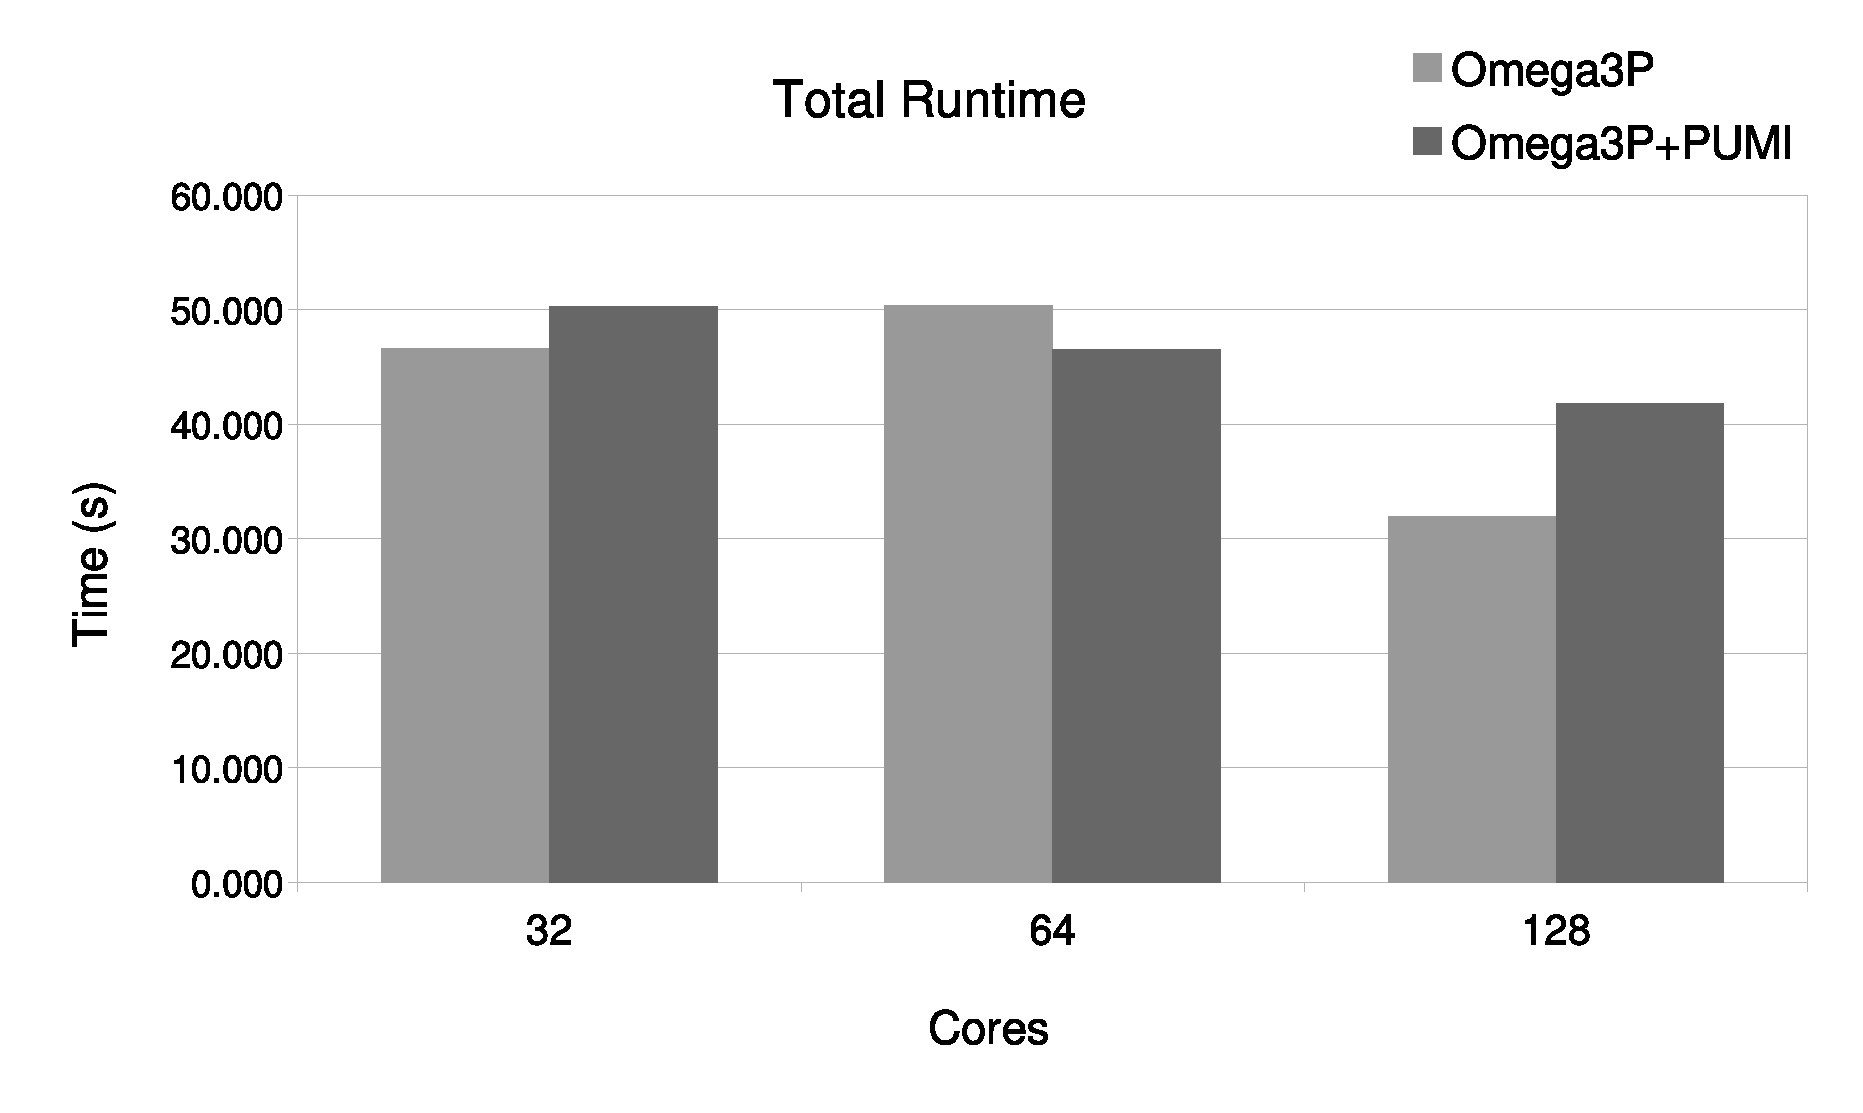
\includegraphics[width=\textwidth]{total-runtime.eps}
  \caption{\label{fig:time} Total runtime averaged over three runs at each core
  count.}
\end{figure}

\begin{figure}[ht]
\centering
  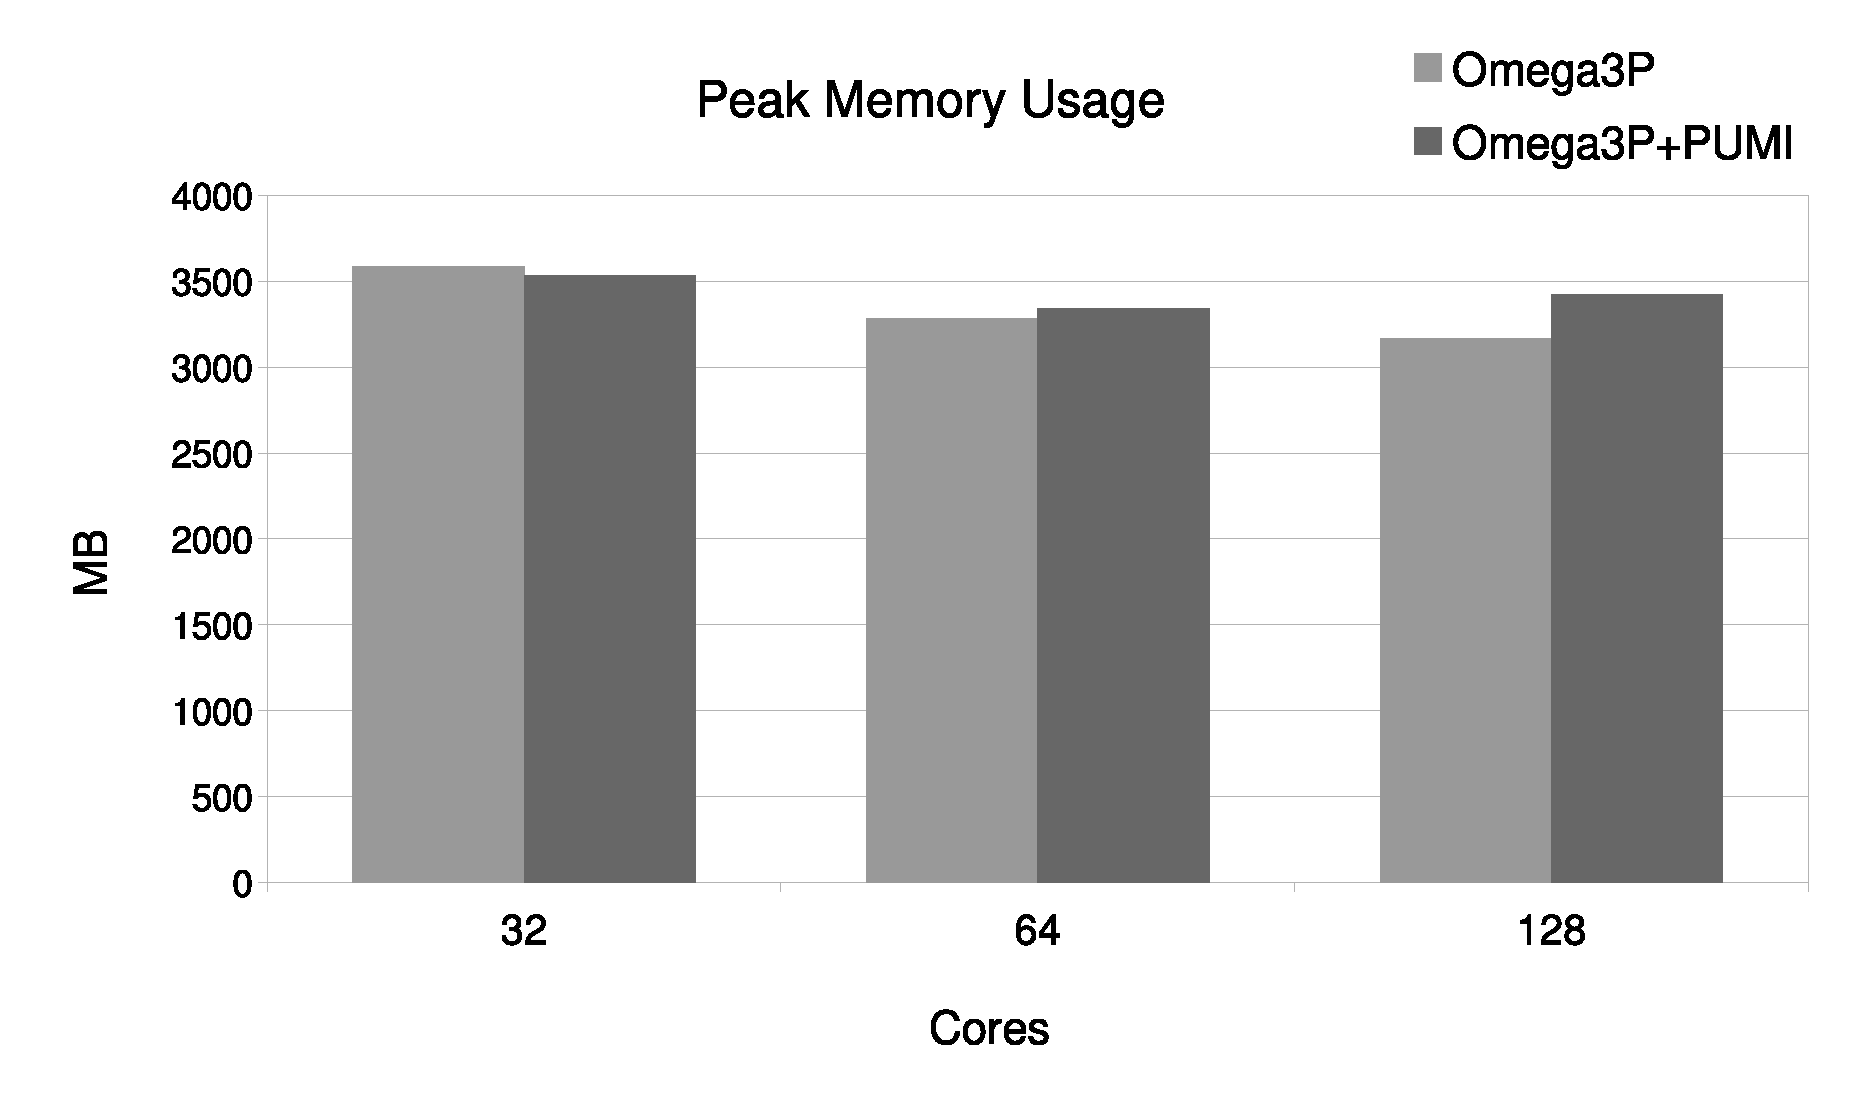
\includegraphics[width=\textwidth]{peak-memory-usage.eps}
  \caption{\label{fig:memusage} Peak memory usage.}
\end{figure}

Our next step will be to perform a detailed analysis of the runtime and memory
usage.
This analysis is expected to confirm initial indications that the imbalance of
ghosted elements is not optimal.
Plans to address the imbalances are described in Section~\ref{sec:lb}.
After we have shown runtime improvements we plan to automate our regression
tests and work with SLAC developers to merge our changes into
the ACE3P central repository and make our documentation accessible.

\newpage \bibliographystyle{plain}
\bibliography{scorec-refs/partition,scorec-refs/meshdb,scorec-refs/hardware,scorec-refs/io,scorec-refs/frameworks,scorec-refs/cr,scorec-refs/fem}

\end{document}


